%% This is emulateapj reformatting of the AASTEX sample document
%%
\documentclass[iop]{emulateapj}

\newcommand{\vdag}{(v)^\dagger}
\newcommand{\myemail}{gbesla@email.arizona.edu}

%%Indicate the beginning of the
%% paper itself with \begin{document}.
\begin{document}


%% LaTeX will automatically break titles if they run longer than
%% one line. However, you may use \\ to force a line break if
%% you desire.

\title{ASTR400B \\
    Example TeX File}

%% Use \author, \affil, and the \and command to format
%% author and affiliation information.
\author{G. Besla\altaffilmark{1} }
\affil{Steward Observatory, U. Arizona, 933 N Cherry Ave, Tucson, AZ, 85721}


%% Mark off your abstract in the ``abstract'' environment. In the manuscript
%% style, abstract will output a Received/Accepted line after the
%% title and affiliation information. No date will appear since the author
%% does not have this information. The dates will be filled in by the
%% editorial office after submission.

\begin{abstract}
A sentence that defines the topic.  A sentence that says why the topic is important. A sentence that says what question you are exploring. A sentence about why that question is important. A sentence that states what you found.
A conclusion about what your finding means. 
\end{abstract}


%%%%%%%%%%%%%%%%%%%%%%%%%%
\section{Introduction}

\begin{enumerate}
	\item  Define the topic you are studying and state why it matters. 
	\item Overview our current understanding of the topic. 
	\item What are the open questions?
	\item Make it clear that you understand the topic!!
\end{enumerate}


%%%%%%%%%%%%%%%%%%%%%%%%%%%%
\section{This Project} 

\begin{enumerate}
	\item State what question(s) you are exploring
	\item Why is this question interesting/important? 
\end{enumerate}


%%%%%%%%%%%%%%%%%%%%%%%%%%%%%
%% In the first two sections, notice the use of the natbib \citep
%% and \citet commands to identify citations.  The citations are
%% tied to the reference list via symbolic KEYs. The KEY corresponds
%% to the KEY in the \bibitem in the reference list below. We have
%% chosen the first three characters of the first author's name plus
%% the last two numeral of the year of publication as our KEY for
%% each reference.
\section{Methods}

\begin{enumerate} 
    
    \item Write a paragraph that describes the simulation you are using. 
    Details can be found in \citet{van12}.  

    \item  Describe the code you wrote. What equations do you use?  
    For example you may have employed some dynamical friction formalism
    \citep[e.g.][]{van12,bes07}.
    
    Here is an example of an equation written in ``math mode":

\begin{equation}
I = \frac{1}{1 + d_{1}^{P (1 + d_{2} )}}
\end{equation}

where

\begin{displaymath}
d_{1} = \sqrt{ \left( \begin{array}{c} \frac{x_{1}}{R_{maj}}
\end{array} \right) ^{2} +
\left( \begin{array}{c} \frac{y_{1}}{R_{min}} \end{array} \right) ^{2} }
\end{displaymath}
\begin{displaymath}
d_{2} = \sqrt{ \left( \begin{array}{c} \frac{x_{1}}{P R_{maj}}
\end{array} \right) ^{2} +
\left( \begin{array}{c} \case{y_{1}}{P R_{min}} \end{array} \right) ^{2} }
\end{displaymath}
\begin{displaymath}
x_{1} = (x - x_{0}) \cos \Theta + (y - y_{0}) \sin \Theta
\end{displaymath}
\begin{displaymath}
y_{1} = -(x - x_{0}) \sin \Theta + (y - y_{0}) \cos \Theta
\end{displaymath}

    \item This code must be unique to you - you cannot simply use the assignment solutions. 
    But you can use the solutions as a starting point to create your code. 
\newline

\end{enumerate}
	
	
%%%%%%%%%%%%%%%%%%%%%%%%%%%%%%%%%%
\section{Results}

\begin{enumerate}
	\item At least one plot should be illustrated (with proper labels and figure caption).  
    
    \item Describe what your code returned. What did you find? Describe what is  in the plot.
    
    Example Plot is provided in figure~\ref{fig:Panorama}:  
    
\begin{figure*}
\begin{center}
\mbox{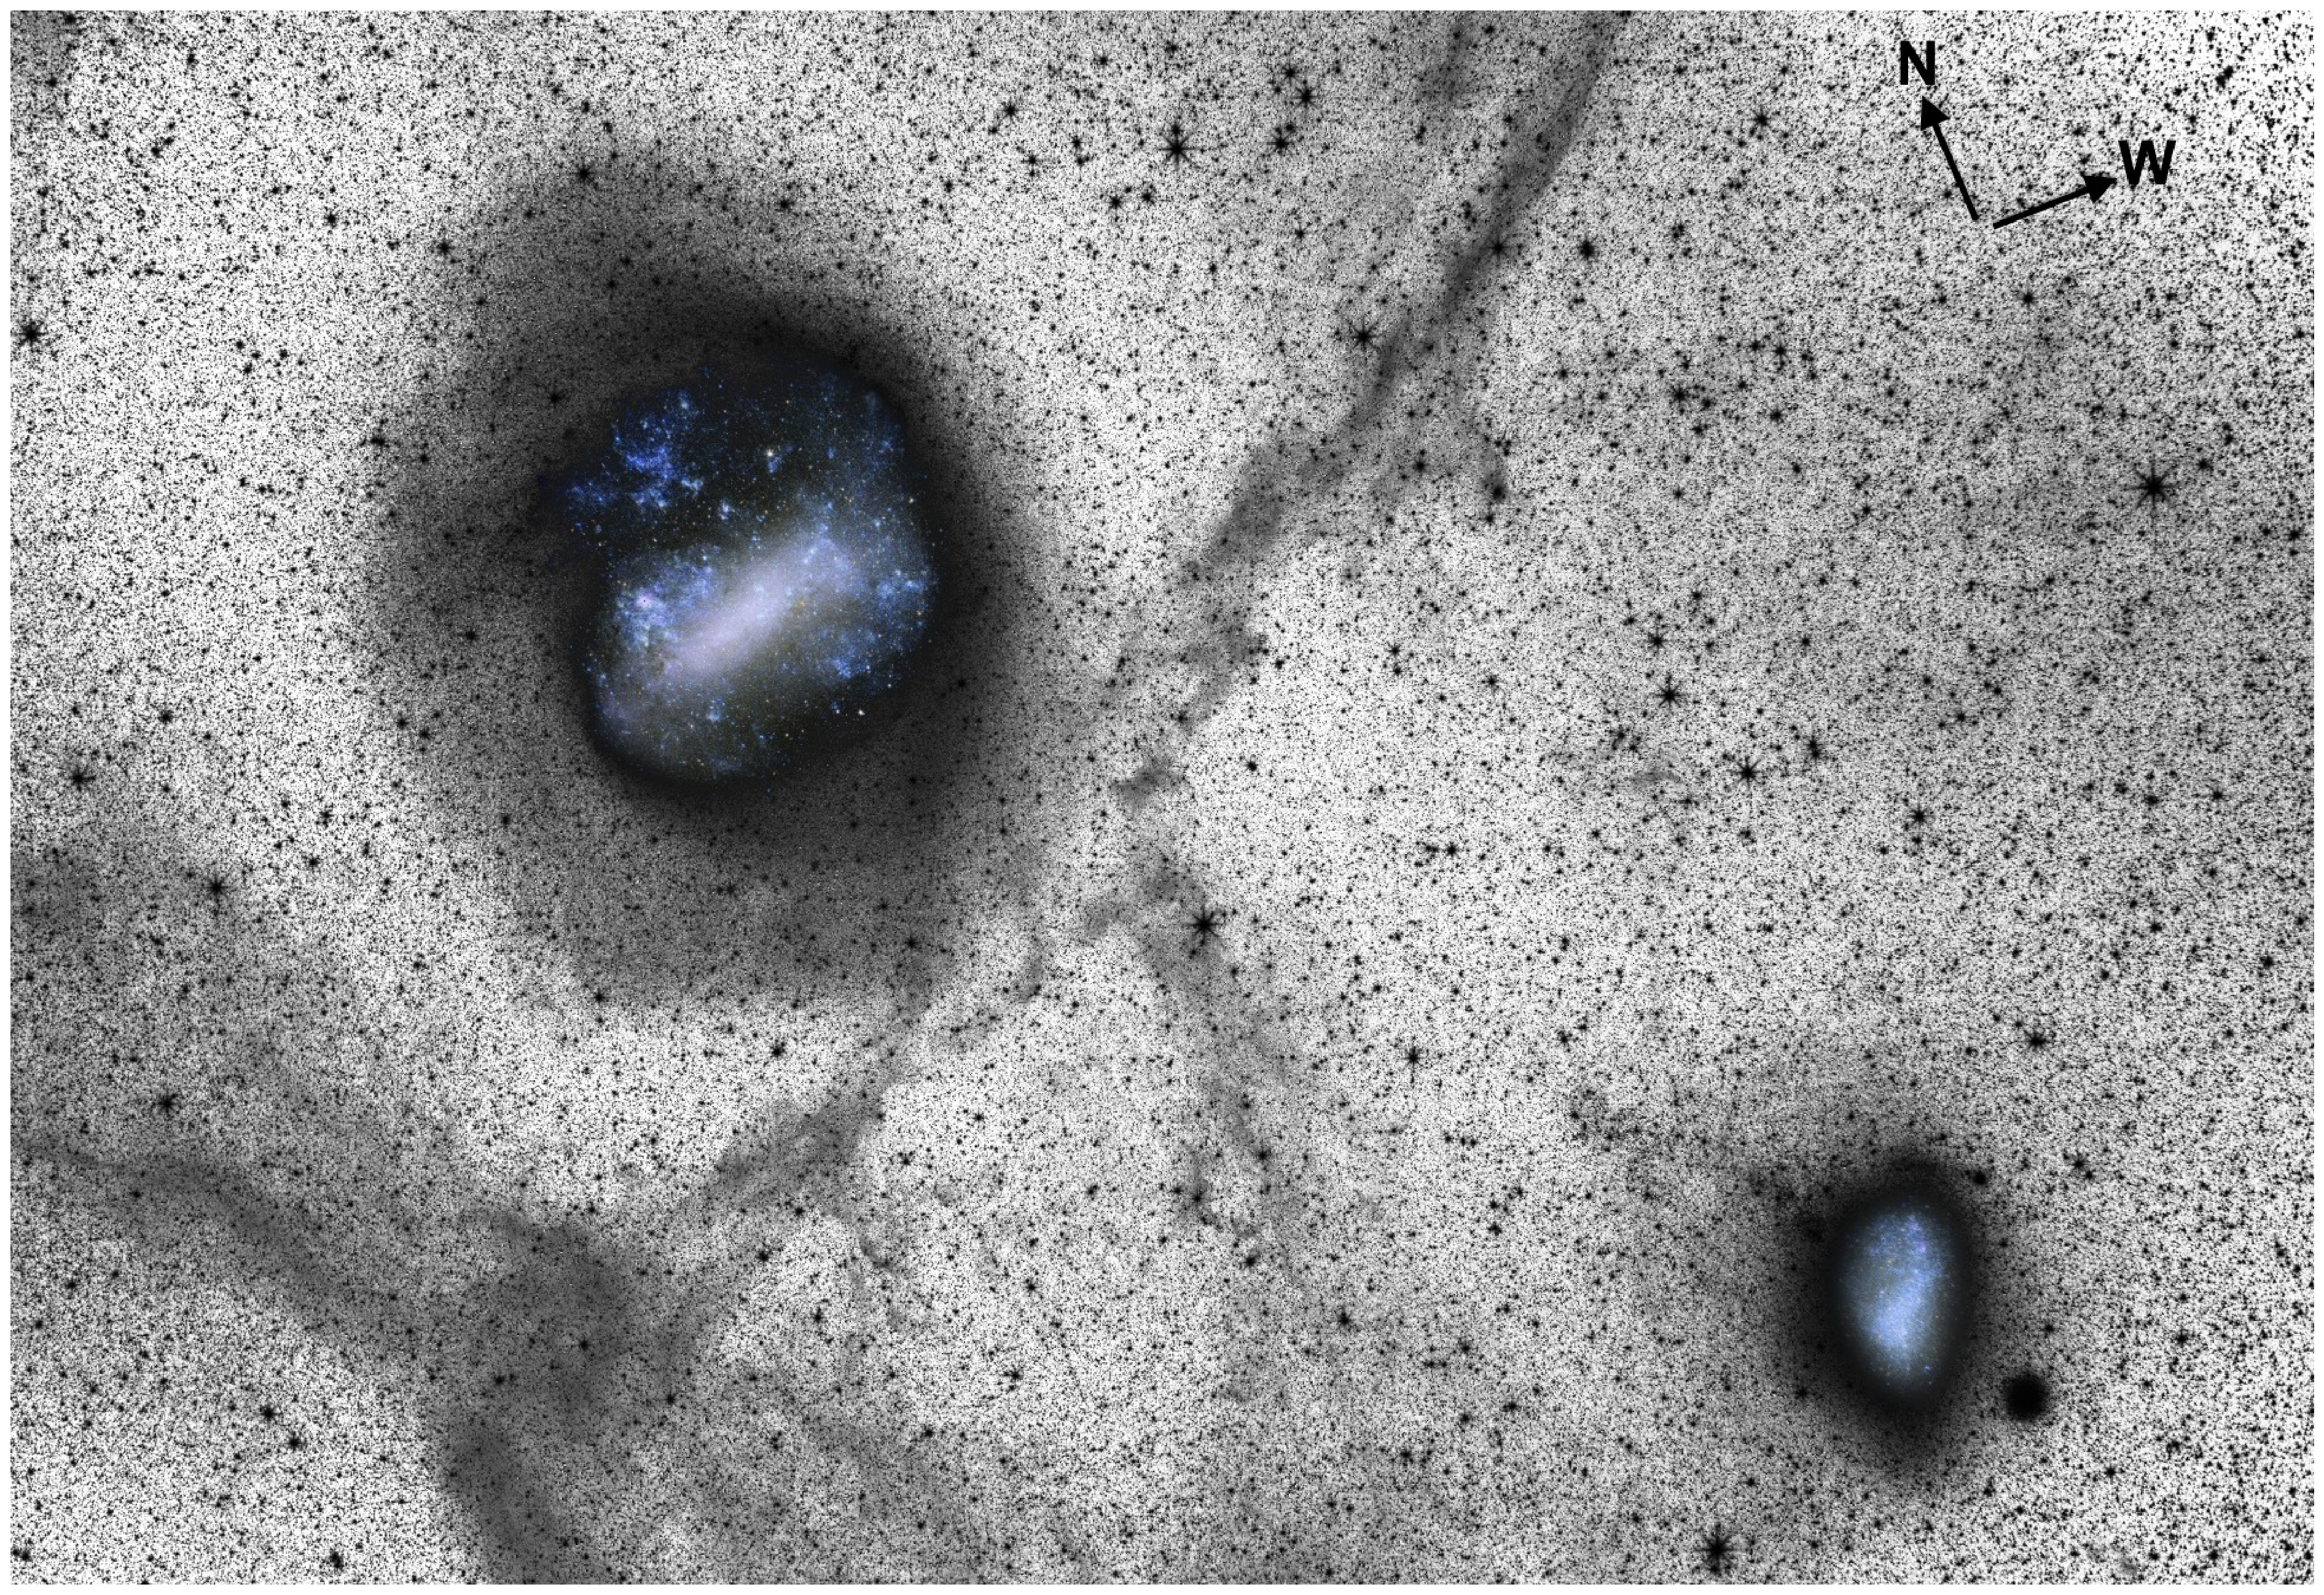
\includegraphics[width=7in]{./Fig1.eps}}
\end{center}
\caption{\label{fig:Panorama} Wide-field Luminance filter image of the 
Magellanic System (39 x 27 degrees). The LMC is located towards the top left 
and the SMC is to the bottom right. The Milky Way globular cluster 47 Tuc is visible to the West of the SMC.A tail of stars from the SMC is visible stretching towards the LMC in the East.  The outskirts of the LMC disk display pronounced asymmetries.  For illustrative purposes, a color inset of the inner regions of the LMC and SMC, made from the color data obtained in our observing run is inserted as a reference and for comparison with previous studies. }
\end{figure*}
    
    
    
\end{enumerate}


%%%%%%%%%%%%%%%%%%%%%%%%%%%%%%%%%%%%%%%%%%
\section{Discussion}

What did you learn?  What do your results mean? What is the importance of your results ? 


%%%%%%%%%%%%%%%%%%%%%%%%%%%%%%%%%%%%%%%%%%	
\section{Conclusion}

\begin{enumerate}
    \item Summarize the paper. Make sure there is a concise summary of what is in each section of the report. 
    
    \item Comment on future directions - what other things could you do to
    explore the topic further? 
    
\end{enumerate} 


%%%%%%%%%%%%%%%%%%%%%%%%%%%%%%%%%%%%%%%%%%%%%
\begin{thebibliography}{}
\bibitem[Besla et al.(2007)]{Bes07} Besla, G., Kallivayalil, N., Hernquist, L., Robertson, B., Cox, T.J., van der Marel, R.P., \& Alcock, C. 2007, \apj, 668, 949
\bibitem[van der Marel et al.(2012)]{van12} van der Marel, R. P., Besla, G., Cox, T. J., Sohn, S.T., \& Anderson, J. 2012, \apj, 753, 9
\end{thebibliography}


 



\end{document}